\section{ACE-M2 Run 4: comparing time evolution among wells with the same sample}\hypertarget{ace-m2-run-4-comparing-time-evolution-among-wells-with-the-same-sample}{}\label{ace-m2-run-4-comparing-time-evolution-among-wells-with-the-same-sample}
The main purpose of Run 4 for ACE-M2 is to observe the time evolution of phase
separating samples in platter 2105, which has five wells all with sample 21 plu\_ACEM2\_lg\_ps, the
phase-separating colloid-polymer mixture using the larger particles. We know
from the comprehensive survey in Run 2 that these samples visibly phase
separate, so the goal is to look at the different wells and see if they all
behave the same---as they should, given that the sample is identical. There may
be some minor variations due to slightly different bubble size and/or mixing by
the crew, but overall we expect similar evolution and structure.

\subsection{Strips 608 and 613: samples A1, C3, C4 and C5}\hypertarget{strips-608-and-613-samples-a1-c3-c4-and-c5}{}\label{strips-608-and-613-samples-a1-c3-c4-and-c5}
As we are standardizing on procedures, we first image the entire well with a 10x
composite tiling at a depth of 80 microns, which for samples A1, C3, C4 and C5
are pretty much the same:
\begin{figure}
\begin{center}
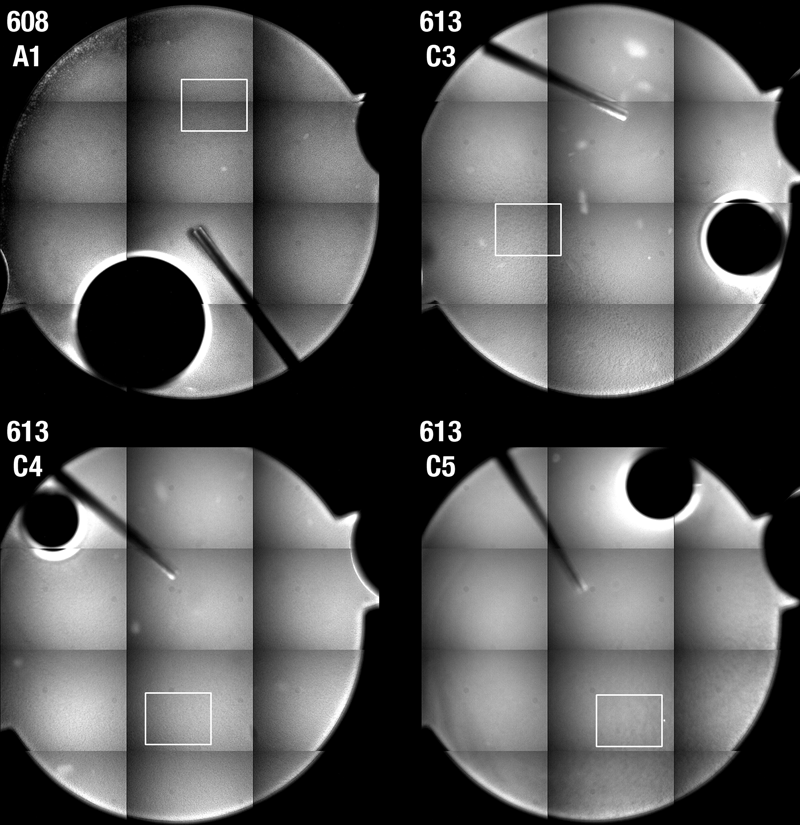
\includegraphics[width=\columnwidth]{./images/2014_07_14_ace_m2_run4/A1_C345_80uM_run4_web.png}
\end{center}
\caption{four similar phase-separating samples A1, C3, C4 and C5}
\end{figure}

The wells look mostly well-mixed, with a small amount of phase separation
visible as the texture in the images develop. But the feature size of the
separation is similar in all wells, so this is suggests we are being consistent
in loading, mixing and imaging.

\subsection{Strip 618: sample B5}\hypertarget{strip-618-sample-b5}{}\label{strip-618-sample-b5}
By contrast, sample B5 is completely different. There is some structure forming,
which is at a much larger length scale: uniformly far more coarse, throughout
the sample well.
\begin{figure}
\begin{center}
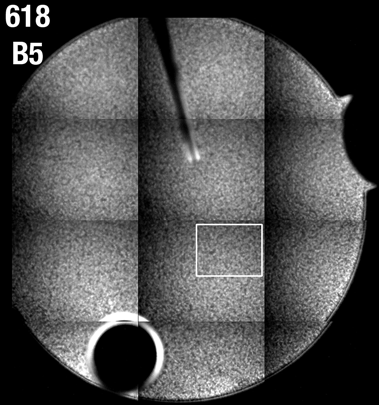
\includegraphics[width=\columnwidth]{./images/2014_07_14_ace_m2_run4/B5_80uM_run4_web.png}
\end{center}
\caption{different-looking phase-separating sample B5}
\end{figure}

This differs significantly from the other four wells, and there is no obvious
scientific reason that we should expect this. Hopefully we will be able to
resolve this mystery with more data as it is collected.